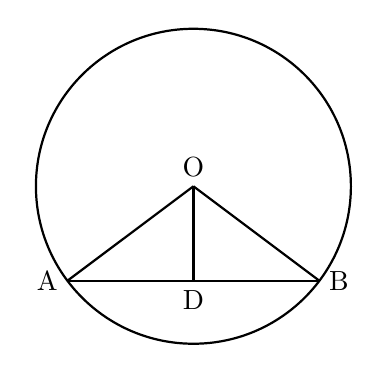
\begin{tikzpicture}[scale=1]

    % Define the center coordinate of the circle
    \coordinate (O) at (0,0);
    
    % Draw the main circle with a radius of 2cm
    \draw[thick] (O) circle (2cm);
    
    % Define coordinates for points A, B on the circle and D on the chord
    % Assuming a radius of 2, the chord AB is placed at y = -1.2 for visual similarity
    % The x-coordinates for A and B are +/- sqrt(2^2 - 1.2^2) = +/- 1.6
    \coordinate (A) at (-1.6, -1.2);
    \coordinate (B) at (1.6, -1.2);
    \coordinate (D) at (0, -1.2);

    % Draw the line segment AB (the chord connecting A and B)
    \draw[thick] (A) -- (B);

    % Draw the line segments OA and OB (radii forming the triangle)
    \draw[thick] (O) -- (A);
    \draw[thick] (O) -- (B);

    % Draw the line segment OD (altitude from center to the chord)
    \draw[thick] (O) -- (D);

    % Add text labels exactly where they appear in the image
    \node[above] at (O) {O};
    \node[left] at (A) {A};
    \node[right] at (B) {B};
    \node[below] at (D) {D};

\end{tikzpicture}